\section{Τεχνολογική στοίβα} \label{section:3-2-technology-stack}

% TODO: Add React/ Redux

\subsection{Ethereum}

Ξεκινώντας την σχεδίαση της πλατφόρμας πραγματοποιήσαμε έρευνα ώστε να ανακαλύψουμε τις πιθανές επιλογές για το κομμάτι της διανεμημένης επεξεργασίας (\textenglish{distributed computing}). Αναλογιστήκαμε τα προτερήματα και μειονεκτήματα διάφορων επιλογών, συμπεριλαμβανομένων των ... 

Επιλέξαμε να προχωρήσουμε με το Ethereum και όχι κάποια άλλη πλατφόρμα επειδή ...


\subsection{IPFS, OrbitDB}

Όπως η επιλογή του Blockchain, που περιγράφηκε στο προηγούμενο κεφάλαιο (\textenglish{insert reference}), ομοίως και η επιλογή του λογισμικού που θα χρησιμοποιηθεί για την κατανεμημένη αποθήκευση δεδομένων ξεκίνησε με μία έρευνα των επιλογών που υπάρχουν. Αναλογιστήκαμε τα προτερήματα και μειονεκτήματα διάφορων επιλογών, συμπεριλαμβανομένων των ... 

Επιλέξαμε να προχωρήσουμε με το IPFS και την OrbitDB έναντι άλλων λύσεων επειδή ...

Η OrbitDB είναι ... και χρησιμοποιεί το IPFS για να καταφέρει τα εξής χαρακτηριστικά ...
Περιορισμοί πάλι κλπ ....

\begin{figure}[H]
    \centering
    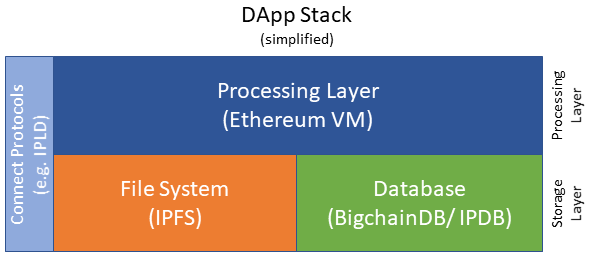
\includegraphics[width=.75\textwidth]{assets/figures/chapter-3/simple_dapp_stack}
    \caption{Τεχνολογική στοίβα}
\end{figure}
